
\section{Introduction}
% no \IEEEPARstart
% You must have at least 2 lines in the paragraph with the drop letter
% (should never be an issue)

  With the vast involvement of stream big data (e.g., stock market data, sensor data, social network data, etc.), quickly mining and analyzing stream big data is becoming more and more important. Many distributed stream processing frameworks such as Storm \cite{storm-web}, Naiad \cite{Murray2013}, S4 \cite{Neumeyer2010}, TimeStream \cite{Qian2013}, ELF \cite{Hu2014} have been developed to meet the requirements of big data real time processing. Batched stream processing systems like HOP \cite{Condie2010}, Comet \cite{He2010}, HStreaming \cite{HStreaming} and Spark Streaming \cite{Zaharia2013} are widely adopted because these systems fully leverage the fault tolerance and high throughput properties of batch framework\cite{spark-summit}. They propose to treat streaming workloads as a series of short batch jobs on small batches of streaming data, using batch processing engine such as MapReduce \cite{Dean2004}, Spark \cite{Zaharia2010C} to process micro-batch jobs.

  Figure 1 illustrates a simple batched stream processing model. The \emph{batching model} is responsible for receiving and dividing the data streams into batches. Then, these batches are put into the \emph{batch queue}. The \emph{processing model} schedules jobs and tasks for processing. Batched stream processing follows the well-known bulk synchronous parallel (BSP) model, where the job must wait until all the tasks complete. However, task execution time varies due to many negative factors, resulting in stragglers. In practice, straggler happens frequently and has been regarded as a major hurdle in achieving fast completion of latency-sensitive applications. In the production clusters at Facebook and Microsoft Bing, straggler tasks are on average 8 times slower than the median task in that job \cite{Ananthanarayanan2013} \cite{Yadwadkar2014}. Stragglers impacts the performance of small batched streaming jobs severely. On the one hand, small batched streaming jobs typically run all their tasks at less waves. Therefore, if one task is straggling, the whole job is significantly delayed. On the other hand, small batched streaming jobs are critically latency-sensitive. Straggling tasks will impact subsequent jobs' submission and execution. Therefore, mitigating or even eliminating stragglers remains a great challenge in batched stream processing.
  \begin{figure}[htbp]
    \centering
    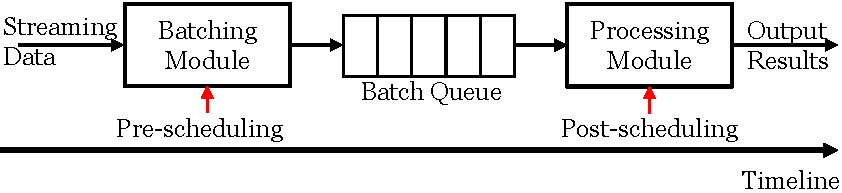
\includegraphics[width=0.40\textwidth]{FigureModel}
    \caption{Model of a batched stream processing system}\label{Fig. 1:}
  \end{figure}

  Much effort has been devoted to migrating the stragglers. Existing representative straggler mitigation techniques are all post-scheduling and can be generally classified into two categories, i.e., reactive and proactive. These techniques are natively developed for batch processing which has large job and task size. However, batched stream processing consists of a number of micro jobs and tiny tasks. They are more latency sensitive. Traditional post-scheduling methods are not suitable for batched stream processing. Reactive ways rely on a wait-speculate-re-execute mechanism, thus leading to delayed straggler detection and inefficient resource utilization. Proactive technique with replication such as Dolly \cite{Ananthanarayanan2013} incurs extra resources. Another proactive technique without replication such as Wrangler \cite{Yadwadkar2014} is also slow as it needs to migrate data at runtime. Existing post-scheduling straggler mitigation approaches suffer from either high resource overhead for task replication or long task completion time due to delayed straggler detection, resulting in the inefficiency for batched stream processing.

  Fortunately, batched streaming processing jobs which are run periodically as new data becomes available \cite{Zaharia2013} are recurring with predictable characteristics, allowing us to carefully optimize the assignment of job input data before scheduling to avoid straggler. These job characteristics include input data distribution, straggler, task execution time, resource utilization and so on. Using these characteristics, we can plan ahead and pre-schedule how to allocate input data and task among nodes with different capability. It is expected that potential stragglers can progress as the same speed as others. Besides, better data locality can be also achieved by coordinating such data assignment with task placement on each node beforehand.

  With this intuition, we present Lever, a pre-scheduling straggler mitigation framework that exploits the predictability of recurring batched stream jobs to optimize the assignment of data. First, Lever observes and collects statistical information of previous jobs(e.g., task completion time on each node, the amount of data processed in previous jobs) when recurring jobs execute over time. Second, Lever identifies potential stragglers and evaluates node's computational capability by analyzing information from previous repetitions, then makes a capability-aware pre-scheduling plan about how to allocate data between each node. Finally, Lever uses this pre-scheduling plan as guidelines to repartition and dispatch input data in data receiving phase.

  In summary, this paper makes the following contributions:
\begin{itemize}
  \item We discuss the behaviors of existing straggler mitigation methods and identify the problems of existing straggler mitigation methods for batched stream processing systems.

  \item To better mitigate stragglers when processing small jobs, we present a pre-scheduling straggler mitigation framework named Lever which leverages the predictability of recurring jobs to pre-schedule input data.

  \item We implement a prototype of Lever based on Spark Streaming and verify its effectiveness through detailed evaluation. We also have contributed Lever as an extension of Apache Spark Streaming to the open source community. The experiments show that Lever can mitigate stragglers efficiently and improve the performance of stream applications significantly.
\end{itemize}

  The rest of this paper is organized as follows. In Section II, we introduce the background and analyze the straggler problems in batched stream processing system. Section III describes the pre-scheduling strategy and the design of Lever. Section IV presents the implementation of Lever. We evaluate the performance of our system in Section V. Section VI briefly surveys the related works. Finally, Section VII concludes this paper.